% =====================================================================
\section{Introduction}\label{sec:intro}
% =====================================================================

\subsection{Does noise make forgetting decidable?}

A probabilistic cellular automaton updates every site of a lattice at once, each site reading a finite neighbourhood through one fixed table of probabilities. When every entry of that table is positive, the automaton has \emph{positive rates}: no value is ever forbidden at any site. Run such an automaton from two different configurations. Does it eventually forget where it started? If it does, from every start, it is \emph{ergodic}: it has one invariant measure, and every initial law converges to it.

For deterministic rules and for rules with forbidden transitions, the answer can encode any computation, and it is undecidable. Kurdyumov \cite{Kurdyumov78} and Toom \cite{Toom00} proved that ergodicity of probabilistic cellular automata cannot be decided by any algorithm, using rules in which some transitions have probability zero; see also \cite{BMM13} for deterministic rules on $\Z$. Positive rates were the natural escape hatch. Noise blurs every configuration, and one may hope that it also blurs away the fine structure that lets an automaton simulate a Turing machine. Toom \cite{Toom80} and G\'acs \cite{Gacs01} showed that noise does not always erase memory: there are positive-rate automata that are not ergodic. Marsan, Sablik and T\"orm\"a \cite{MarsanSablikTorma26} gave a perturbed automaton with two phase transitions for ergodicity. Marcovici, Sablik and Taati \cite{MST19} studied which noisy automata are ergodic, and Marcovici and Taati \cite{MT26} proved that, at one fixed positive rate, automata with a stationary Bernoulli measure cannot be computably separated from those without one. Whether ergodicity itself remains undecidable at a fixed positive noise rate is the question of this paper.

The answer is that it does. Noise does not make forgetting decidable.

\begin{mainA}[\cref{thm:main,cor:eight}]
There is a total computable map $M\mapsto R_M$ from Turing machines to finite Wang sets with the following property. Put $\eps_0=490000^{-99}$. For every $\eps\in(0,\eps_0]$, the quorum rule of $R_M$ on $\Z^{8}$, followed by uniform random replacement at rate $\eps$, is a positive-rate probabilistic cellular automaton that is ergodic if and only if $M$ halts.
\end{mainA}

The rule, the noise and the rate are explicit (\cref{sec:setting,fgt:rem-constants,cor:eight}). Every member of the family has positive rates, and the noise is the same uniform replacement at the same rate for every member. \Cref{cor:eight}, which is Theorem~A on $\Z^8$, and the statement that ergodicity in the family is undecidable are proved in the proof assistant Lean~4 with the Mathlib library (\cref{app:lean}).

\subsection{How it works: a team of inspectors}

The automaton is built from a Wang tile set $R$ \cite{Wang61}. Each site holds a legal $3\times3$ block of tiles and a check bit, or a blank symbol $\bot$. A checker erases every block that disagrees with a neighbour, and a quorum over $k$ extra copies of the plane restores what most copies agree on (\cref{set:def-quorum}). Two theorems tie the behaviour of this noisy rule to a property of $R$.

Picture $j$ inspectors walking on the plane. Each one sees a $3\times3$ patch and may step to a neighbouring site or jump onto another inspector; together they try to corner a contradiction in the tile rules. The bookkeeping of what they can still believe is a finite deletion procedure, which we call the $j$-token tables (\cref{sec:setting}). When the tables empty, the team has refuted $R$, and we say $R$ is \emph{$j$-token refutable}. In the language of constraint satisfaction, the team wins whenever Spoiler wins the existential $j$-pebble game \cite{KolaitisVardi00,ABD07}, and a win of the team is a win of Spoiler with $j+1$ pebbles in the game where Duplicator answers with $3\times3$ blocks (the live target of \cref{thm:game}): a refutation of bounded width.

\begin{mainB}[\cref{thm:memory,thm:forgetting}]
Fix $j\ge1$, $k\ge\max(2,2j)$ and $0<\eps\le\eps_k$, where $\eps_k$ is the explicit rate of \cref{fgt:rem-constants}. For every finite Wang set $R$:
\begin{enumerate}[label=\textup{(\roman*)}]
\item if $R$ tiles the plane, the noisy quorum rule of $R$ remembers a bit forever and is not ergodic;
\item if $R$ is $j$-token refutable, the noisy quorum rule of $R$ forgets its initial configuration exponentially fast after a delay set by the refutation, and is ergodic.
\end{enumerate}
\end{mainB}

Part (i) is a Toom-type stability argument \cite{Toom80,SST26}. Part (ii) is the new mechanism: every failed relation among $j$ inspectors is covered by a field that depends on the noise alone, and contours of that field force linearly many distinct noise events along any path that carries a discrepancy. The bounded width of the refutation is what lets a quorum transport it through noise. A refutation needing an unbounded number of inspectors would give no such cover.

The two parts leave a gap: a tile set that does not tile but needs ever more inspectors to refute. If every undecidable family of tile sets fell into that gap, Theorem~B would decide nothing. The third theorem closes the gap.

\begin{mainC}[\cref{thm:width,thm:three}]
There is a total computable map $M\mapsto R_M$ to finite Wang sets such that $R_M$ tiles the plane if and only if $M$ does not halt, and $R_M$ is $3$-token refutable whenever $M$ halts.
\end{mainC}

So a team of three inspectors can always find the flaw, yet nobody can tell in advance whether there is one. The construction has two halves, and each is chosen so that bounded width suffices for it. The geometry is a fixed hierarchical tiling, Ollinger's $2\times2$ substitution \cite{Ollinger08}, in the transcription of \cite{LeanWang}, decorated with ruler bits. Recognizability lets a bounded number of inspectors read the type of a supertile of any size, through certificates of bounded treewidth \cite{Mosse92,Solomyak98,DKV02}. The computation runs in a layer of Horn clauses. Constraints closed under intersection are decided by local consistency alone \cite{JCG97,FederVardi98}, so once the geometry is pinned, the inspectors can reconstruct a whole computation square from pairwise checks. \Cref{sec:scaffold,sec:family,sec:refutation} carry this out with a large fixed number of inspectors; \cref{sec:three} shows that three suffice for the same family, two holding the phase of the hierarchy while the third walks. Theorem~A follows by applying Theorem~B to the family of Theorem~C with $k=\max(2,2j)$, which is $6$ for $j=3$ (\cref{sec:proofs,cor:eight}).

\subsection{Consequences}

The proof has further consequences (\cref{sec:forgetting,sec:proofs}).
\begin{itemize}
\item \emph{One family for every small rate.} The conditions on $\eps$ in Theorem~B are monotone, so the same family works at every rate in $(0,\eps_0]$ (\cref{cor:rates}). Other replacement laws work as well (\cref{cor:laws}).
\item \emph{A whole neighbourhood of rules.} Every probabilistic cellular automaton whose transition table lies within total-variation distance $\eps_0$ of a member of the family has the same classification: it is ergodic exactly when $M$ halts (\cref{cor:robust}). The radius is the same for every member.
\item \emph{Tiling reduces to forgetting.} A computable map sends every finite Wang set to a noisy automaton, in one fixed dimension and at every rate in $(0,\eps_0]$, that is ergodic exactly when the set does not tile the plane (\cref{cor:tiling}).
\item \emph{Forgetting cannot be timed.} Every halting member forgets, but at every rational rate no computable function of $M$ bounds the time it takes (\cref{cor:mixing}). Otherwise a finite simulation would decide halting.
\item \emph{All starts at once.} The forgetting bound of Theorem~B(ii) holds for all initial configurations at once. Under one realisation of the noise, the value at a site at time $t$ is the same for every start, outside an event that depends on the replacement indicators alone and has probability at most $2\eps^{-\tau/a}\beta^t/(1-\beta)$ (\cref{fgt:coalesce}).
\item \emph{Phase coexistence is undecidable.} A positive-rate automaton defines a translation-invariant, finite-range interaction one dimension up, whose Gibbs measures include the trajectories of the dynamics \cite{GKLM89,DM26}. For our family this interaction has exactly one Gibbs measure, with no invariance assumed, if $M$ halts, and its specification then has exponential weak spatial mixing in arbitrary volumes; if $M$ does not halt, it has at least two translation-invariant Gibbs measures (\cref{cor:gibbs}). So uniqueness of the Gibbs measure, uniqueness of the translation-invariant Gibbs measure and exponential weak spatial mixing are each undecidable on this family. Uniqueness among all Gibbs measures and weak mixing come from the previous item, through a theorem of our paper \cite{DM26} on space-time Gibbs states.
\item \emph{One phase or a continuum.} Running each member on parallel copies, each copy reading the next, gives automata on $\Z^9$ that have one invariant measure if $M$ halts and, if $M$ does not halt, a continuum of invariant measures, each extreme among all invariant measures and mixing in time (\cref{cor:stack}).
\end{itemize}
\Cref{tab:summary} lists the properties that coincide with halting on the family.

\begin{table}[ht]
\centering\small
\begin{tabularx}{\textwidth}{@{}>{\raggedright\arraybackslash}X>{\raggedright\arraybackslash}p{3.3cm}>{\raggedright\arraybackslash}p{3.3cm}>{\raggedright\arraybackslash}p{2.2cm}@{}}
\toprule
Property of the member & $M$ halts & $M$ runs forever & Proved in\\
\midrule
Ergodic & yes; $\delta_O(t)\le4|O|\eps^{-\tau/a}2^{-t}$ & no; memory with amplitude $1-2.02\eps$ & Theorem~A\\
Time to forget & finite, not computably bounded & infinite & \cref{cor:mixing}\\
Gibbs measures of the space-time interaction & exactly one & at least two translation-invariant ones & \cref{cor:gibbs}\\
Exponential weak spatial mixing & yes & no & \cref{cor:gibbs}\\
Invariant measures of the stacked automaton & exactly one & an arc of extreme ones & \cref{cor:stack}\\
\bottomrule
\end{tabularx}
\caption{What coincides with halting on the family, at every rate $\eps\in(0,\eps_0]$. Each property in the first column is therefore undecidable on the family. Here $\delta_O(t)$ measures how far the law at time $t$ on a window $O$ still depends on the start (\cref{set:def-forget}), and $\tau$ is the refutation time of $R_M$.}
\label{tab:summary}
\end{table}

\subsection{Objections answered}

\paragraph{The dimension.} Theorem~A holds on $\Z^8$ (\cref{cor:eight}). One inspector never suffices (\cref{set:one-token-family}); two would place Theorem~A on $\Z^6$, where the forgetting theorem applies with $k=4$. Whether two suffice is the first question of \cref{sec:discussion}.

\paragraph{The alphabet grows with the machine.} Each member of the family has its own finite alphabet, so the smallest transition probability, $\eps$ divided by the alphabet size, is not bounded below over the family. ``A fixed noise rate'' means the same replacement rate $\eps$, with uniform replacement, for every member. This is the setting of the question above and of \cite{MT26}.

\paragraph{Borderline members.} Is the undecidability caused by members close to a phase boundary? No. Every halting member forgets exponentially fast, with a decay factor $2^{-t}$ that does not depend on $M$, and every other member has memory with amplitude $1-2.02\eps$. No algorithm separates these two kinds, even when it is promised that the given member is of one of them (\cref{sec:proofs}).

\paragraph{Is this the classical reduction with noise added?} No. The classical reductions \cite{Kurdyumov78,Toom00} keep a computation exact because some transitions never happen. Here every transition happens. The undecidability survives because the dichotomy of Theorem~B is itself stable under noise: memory from tilings, forgetting from bounded-width refutations, at one rate chosen before the tile set.

\subsection{Reading guide}

\Cref{sec:setting} defines the automaton, the noise and the token tables, and relates refutations by tokens to refutations in the existential pebble game. \Cref{sec:forgetting,sec:memory} prove the two halves of Theorem~B; a reader interested only in the noise can stop there. \Cref{sec:scaffold,sec:family,sec:refutation} prove Theorem~C: the hierarchical scaffold and its parser, the routing of a machine onto the scaffold, and the bounded-width refutation of every halting member. \Cref{sec:three} lowers the number of tokens to three, which gives Theorem~A on $\Z^8$; one finite lemma there is checked by computer. \Cref{sec:forgetting} ends with the form of the forgetting bound that holds for all starts at once (\cref{fgt:sec-all}). \Cref{sec:proofs} assembles Theorem~A and proves the corollaries, among them the equilibrium consequences (\cref{cor:gibbs}) and the stacked automata (\cref{pf:sec-stack}), and \cref{sec:discussion} lists open problems. The explicit tile tables are in \cref{app:tables}, the one-sided machine used by the construction is in \cref{app:machine}, and \cref{app:lean} describes the formal proof of Theorem~A on $\Z^8$.

\begin{figure}[ht]
\centering
\resizebox{\textwidth}{!}{%
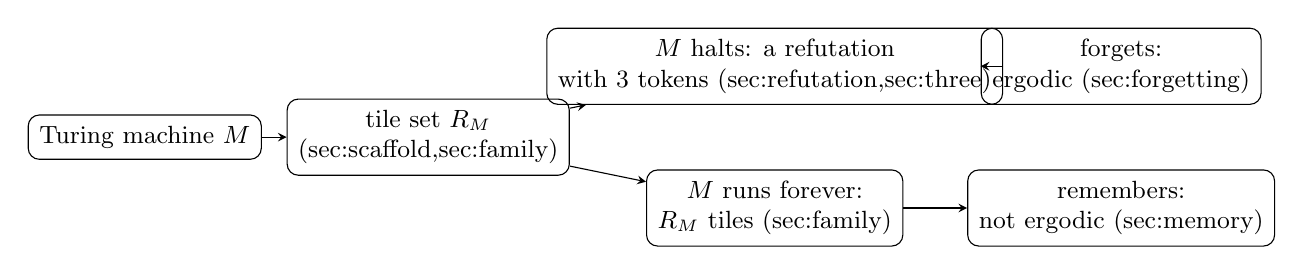
\begin{tikzpicture}[box/.style={draw,rounded corners,align=center,font=\small,inner sep=4pt},>=stealth]
\node[box] (M) at (0,0) {Turing machine $M$};
\node[box] (R) at (3.6,0) {tile set $R_M$\\(\cref{sec:scaffold,sec:family})};
\node[box] (H) at (8.0,0.9) {$M$ halts: a refutation\\with $3$ tokens (\cref{sec:refutation,sec:three})};
\node[box] (N) at (8.0,-0.9) {$M$ runs forever:\\$R_M$ tiles (\cref{sec:family})};
\node[box] (E) at (12.4,0.9) {forgets:\\ergodic (\cref{sec:forgetting})};
\node[box] (F) at (12.4,-0.9) {remembers:\\not ergodic (\cref{sec:memory})};
\draw[->] (M) -- (R);
\draw[->] (R) -- (H);
\draw[->] (R) -- (N);
\draw[->] (H) -- (E);
\draw[->] (N) -- (F);
\end{tikzpicture}}
\caption{The proof of Theorem~A. The same noisy quorum rule, at the same rate, is built from $R_M$ in both cases.}
\label{fig:chain}
\end{figure}
